\section{消融实验、代码保真度与 PCT 诊断性案例研究}
\label{sec:code_audit}

检验物理约束的实证主张，需要同时裁决已发表消融实验的因果隔离度与公开软件计算图的代数执行保真度。

\subsection{已发表文献消融实验中的因果混淆}
对全量 46 篇文献的深入语义提取表明，仅有 \textbf{50.0\% (23/46)} 的研究执行了真正隔离物理约束的消融实验，详见表~\ref{tab:ablation_semantics}。

\begin{table*}[!t]
\centering
\footnotesize
\renewcommand{\arraystretch}{0.92}
\setlength{\tabcolsep}{3.5pt}
\caption{46 项审计文献中消融实验的语义分类与因果可解释性评估。}
\label{tab:ablation_semantics}
\begin{tabularx}{\textwidth}{p{4.2cm}rrX}
\toprule
\textbf{消融实验语义类型} & \textbf{文献数量 ($N=46$)} & \textbf{占比 (\%)} & \textbf{因果有效性与实证可解释性评估} \\
\midrule
\texttt{约束开闭消融 (on-off)} & 17 & 37.0\% & \textbf{严格物理隔离}：在完全相同的网络架构下严格对比 $\lambda=0$ vs. $\lambda > 0$，因果隔离了物理正则化项。 \\
\texttt{兼具两者 (both)} & 6 & 13.0\% & \textbf{严格物理隔离}：兼具参数隔离测试（$\lambda=0$）与模块结构消融，满足无混淆实验对照准则。 \\
\texttt{粗粒度模块消融} & 23 & 50.0\% & \textbf{混淆参数容量}：直接砍掉整个神经网络子模块（如空间 GNN 分支）；评估的是模块总体容量而非物理先验。 \\
\midrule
\textbf{严格隔离消融文献总数} & \textbf{23} & \textbf{50.0\%} & 现有文献中仅有约半数的研究真正因果隔离了物理约束本身的作用。 \\
\bottomrule
\end{tabularx}
\end{table*}


在另外 50.0\%（23/46）的文献中，所谓“消融实验”直接移除了整个神经网络子模块——例如空间图注意力卷积块、多头跨注意力交互层或信号多尺度分解层。当模型在移除大型 GNN 模块后性能下降时，无法判定该下降源自邻接矩阵中物理方程的缺失，还是源自数以万计可训练参数及多层非线性表征能力的剥离。这种模块级消融评估的是网络架构的综合参数容量，无法构成物理先验因果有效性的独立实证证据。

\subsection{诊断性案例研究：物理约束 Transformer (PCT)}
\label{sec:pct_case}
正如第~\ref{sec:protocol}节所述，在被审计的 46 项研究中，仅有两项公开了软件代码库：PINN-UQ \cite{s10_pinnuq2025} 在代码实现上与其已发表代数关系严格对齐（$\mathcal{D}_4 = \texttt{code-aligned}$，2.2\%），而\textbf{物理约束 Transformer (PCT)} \cite{pct2026}（发表于 \textit{Scientific Reports} 2026 年，DOI: 10.1038/s41598-025-34348-x；官方 GitHub 代码仓库，提交版本 \texttt{65941ec}）是端到端物理约束 Transformer 的唯一公开训练代码库，也是唯一存在代码实现偏差的代码库（$\mathcal{D}_4 = \texttt{divergent-code}$，2.2\%）。为了洞察统计分布物理约束究竟如何在底层软件中落地，我们对 PCT 展开了深入的静态计算图代码审计。

\subsubsection{论文数学公式规范与实际代码执行的代数级失配}
在 PCT 论文的第 2 节中，作者提出通过惩罚历史风速-功率经验联合概率分布（$P_{\text{ref}}$）与模型预测的联合概率分布（$P_{\text{pred}}$）之间的统计差异来正则化网络，并显式给出了标准对称的 \textbf{Jensen--Shannon (JS) 散度}：
\begin{equation}
\begin{aligned}
\mathcal{L}_{\text{JS}}(P_{\text{pred}} \parallel P_{\text{ref}}) &= \frac{1}{2} \text{KL}\left(P_{\text{pred}} \,\Big\|\, \frac{P_{\text{pred}} + P_{\text{ref}}}{2}\right) \\
&\quad + \frac{1}{2} \text{KL}\left(P_{\text{ref}} \,\Big\|\, \frac{P_{\text{pred}} + P_{\text{ref}}}{2}\right),
\end{aligned}
\label{eq:js_divergence}
\end{equation}
其中 $\text{KL}(p \parallel q) = \sum_i p_i \log \frac{p_i}{q_i}$ 为经典的 Kullback--Leibler (KL) 散度。论文强调，JS 散度的对称性与理论有界性（$0 \le \mathcal{L}_{\text{JS}} \le \ln 2$）能够提供数值稳定性并防止梯度爆炸。

对 PCT 官方训练脚本（\texttt{train\_clean.py}，第 349--352 行；提交哈希 \texttt{65941ec}）展开抽象语法树（AST）静态解析，其实际损失计算节点为：
\begin{center}
\small
\begin{minipage}{0.95\columnwidth}
\texttt{loss\_phy = 0.5 * (} \\
\hspace*{1em}\texttt{F.kl\_div(pred\_kde.log(), m\_kde, ...)} \\
\hspace*{1em}\texttt{+ F.kl\_div(true\_kde.log(), m\_kde, ...))}
\end{minipage}
\end{center}
在 PyTorch C++ ATen 内核后端（\texttt{native/Loss.cpp}，实现 \texttt{kl\_div\_backward\_cpu}）中，函数 \texttt{torch.nn.functional.kl\_div(input, target)} 的规范定义为：
\begin{equation}
\begin{aligned}
&\text{\texttt{kl\_div}}(u, v) = \sum_{i} v_i \cdot \big( \log v_i - u_i \big).
\end{aligned}
\label{eq:pytorch_kl}
\end{equation}
将 \texttt{input} 绑定为 $\log p$、\texttt{target} 绑定为 $q$ 时，C++ 内核计算：
\begin{equation}
\begin{aligned}
\text{\texttt{kl\_div}}(\log p, q) &= \sum_{i} q_i \cdot \big( \log q_i - \log p_i \big) \\
&= \text{KL}(q \parallel p).
\end{aligned}
\label{eq:reverse_kl}
\end{equation}
因此，\texttt{train\_clean.py} 构建的计算图实际执行：
\begin{equation}
\begin{aligned}
\mathcal{L}_{\text{code}} &= \frac{1}{2} \text{KL}\left(M \parallel P_{\text{pred}}\right) + \frac{1}{2} \text{KL}\left(M \parallel P_{\text{ref}}\right), \\
\text{其中 } M &= \frac{P_{\text{pred}} + P_{\text{ref}}}{2}.
\end{aligned}
\label{eq:reverse_js}
\end{equation}
公式~\eqref{eq:reverse_js} 定义了\textbf{反向参数的 JS 散度}。该式在 $P_{\text{pred}}$ 与 $P_{\text{ref}}$ 之间保持代数对称。然而，将 KL 散度参数从 $\text{KL}(P \parallel M)$ 颠倒为 $\text{KL}(M \parallel P)$，将优化动力学从模式覆盖（mode-averaging，对 $P$ 求期望并惩罚零覆盖）逆转为模式寻求（mode-seeking，对 $M$ 求期望并对低概率区域施加极端除法惩罚）。在稀疏评估网格或无界支集上，一旦预测概率 $P_{\text{pred}}(i,j) \to 0$ 而混合分布 $M(i,j) > 0$，比值 $M/P_{\text{pred}}$ 发散至无穷大。这彻底破坏了标准 JS 散度的 $[0, \ln 2]$ 有界性保证，在计算图底层重构了物理正则化的损失曲面。

\paragraph{实证优化动力学对比：官方 Reverse-JS 与修正 Standard-JS}
为回答参数调换是否对神经网络训练产生实质影响，我们在 Kelmarsh 与 Penmanshiel 上跨 $\lambda \in \{0.01, 0.1, 1.0\}$ 开展了 5 个随机种子的对比训练实验（图~\ref{fig:pct_contrast}）。实证结果揭示出两大结构性影响：第一，Reverse-JS 诱发了显著的梯度膨胀不稳定现象。在强正则化（$\lambda = 1.0$）下，Reverse-JS 的平均梯度 $L_2$ 范数在 Kelmarsh 达到 $0.1665 \pm 0.0160$、在 Penmanshiel 达到 $0.2465 \pm 0.0217$，相比修正 Standard-JS（分别为 $0.0756 \pm 0.0048$ 与 $0.0907 \pm 0.0067$）呈现出 $2.20$ 倍与 $2.72$ 倍的梯度放大（图~\ref{fig:pct_contrast}a），这一梯度激增源于预测概率逼近支集边界时的 $-\frac{P_{\text{ref}, i}}{4 P_{\text{pred}, i}}$ 逆密度导数奇点（$\mathcal{O}(1/\epsilon)$）。第二，在低惩罚权重（$\lambda = 0.01$）下，修正 Standard-JS 在 Penmanshiel 取得 $0.09804 \pm 0.00024$ 的调度成本（优于无约束基准 $0.09864$），而官方 Reverse-JS 则劣化至 $0.09997 \pm 0.00086$（产生 $+1.35\%$ 的过早性能恶化；图~\ref{fig:pct_contrast}b）。然而，在强正则化（$\lambda=1.0$）下，两种散度变体均劣于无约束基准，修正 Standard-JS 的调度成本升至 $0.10549 \pm 0.00149$，而官方 Reverse-JS 为 $0.10292 \pm 0.00103$。修正参数传递顺序消除了人为的梯度爆炸并防止了弱惩罚下的过早性能劣化，但并不能消除过强物理正则化带来的决策性能损失。

\begin{figure*}[!t]
\centering
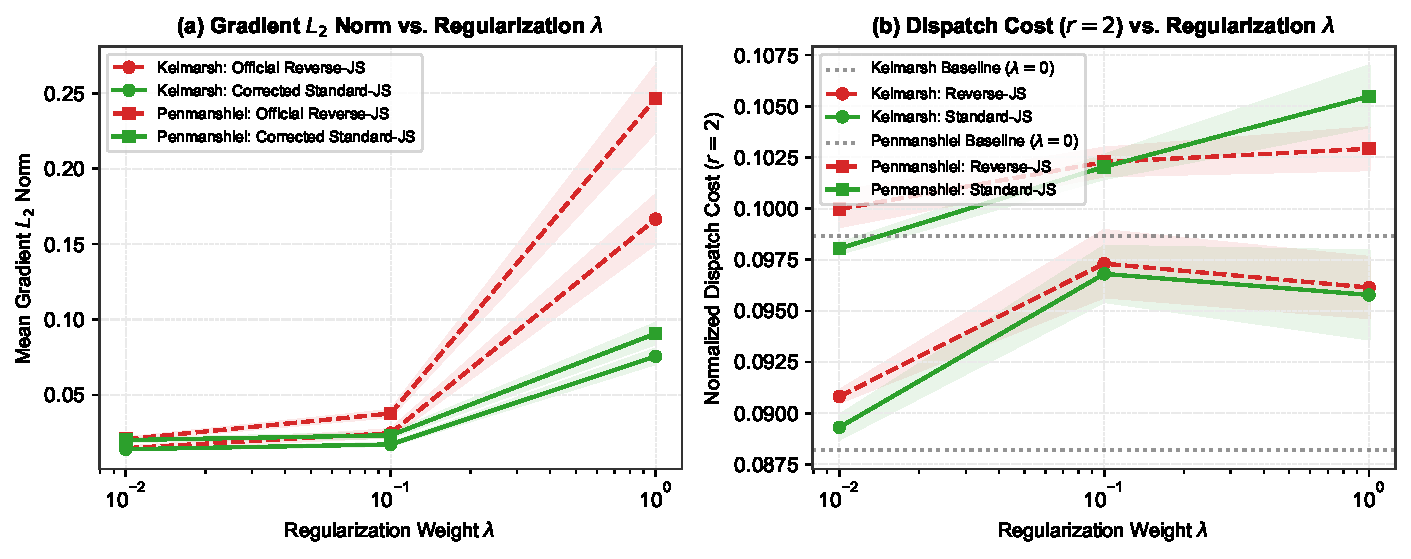
\includegraphics[width=\textwidth]{fig_pct_loss_empirical_contrast.pdf}
\caption{官方 Reverse-JS 与修正 Standard-JS 在跨惩罚尺度 $\lambda \in [0.01, 1.0]$ 下的实证训练对比 (Kelmarsh 与 Penmanshiel, 5 个随机种子均值与标准差)。(a) 平均梯度 $L_2$ 范数：在 $\lambda=1.0$ 下，Reverse-JS 因逆密度奇点引发显著梯度放大（Kelmarsh 2.20倍，Penmanshiel 2.72倍），而 Standard-JS 保持平稳数值有界；(b) 调度决策成本 ($r=2$)：Standard-JS 在低 $\lambda=0.01$ 下防范了过早性能恶化，但在过度强正则化下两种变体均表现出性能衰减。}
\label{fig:pct_contrast}
\end{figure*}

\subsubsection{阴性对照：二维乘积核密度估计的代数严格等价性证明}
阴性对照构成纯形式代数展开，旨在反驳独立性假说。此前针对 PCT 代码库的外部讨论曾提出质疑，猜测其张量外积操作：
\begin{equation}
G = K_p^\top K_w \in \mathbb{R}^{B_p \times B_w}
\label{eq:outer_product}
\end{equation}
假定了风速与功率的统计独立性（$p(w, P) = p(w)p(P)$），进而推断其二维联合密度估计在原理上失效。

形式代数展开证伪了该独立性猜测。设 $\{ (P_s, w_s) \}_{s=1}^N$ 为批次内的成对风速与功率实测样本，$\{b_i^p\}_{i=1}^{B_p}$ 与 $\{b_j^w\}_{j=1}^{B_w}$ 分别代表功率与风速的一维评估网格中心。代码中所计算的一维高斯核向量分别为：
\begin{equation}
\begin{aligned}
\left[K_p\right]_{s,i} &= \phi\left( \frac{b_i^p - P_s}{h_p} \right), \\
\left[K_w\right]_{s,j} &= \phi\left( \frac{b_j^w - w_s}{h_w} \right),
\end{aligned}
\label{eq:kernel_eval}
\end{equation}
其中 $\phi(u) = \frac{1}{\sqrt{2\pi}} e^{-u^2/2}$ 为标准高斯核函数，$h_p, h_w$ 为核窗宽。计算矩阵乘积在网格点 $(i,j)$ 处的元素：
\begin{equation}
\begin{aligned}
\left[ K_p^\top K_w \right]_{i,j} &= \sum_{s=1}^N \left[K_p\right]_{s,i} \cdot \left[K_w\right]_{s,j} \\
&= \sum_{s=1}^N \phi\left( \frac{b_i^p - P_s}{h_p} \right) \cdot \phi\left( \frac{b_j^w - w_s}{h_w} \right).
\end{aligned}
\label{eq:kde_proof}
\end{equation}
公式~\eqref{eq:kde_proof} 在数学上严格等价于相关双变量数据上标准\textbf{成对二维乘积核密度估计器 (2D product-kernel KDE)} 的解析定义。累加求和沿样本索引 $s$ 同步收缩，保留了实测样本 $P_s$ 与 $w_s$ 之间的经验联合耦合。形式代数展开推翻了独立性猜测，确立了张量外积操作忠实执行了双变量联合估计。
